\documentclass[12pt]{article}
\usepackage[utf8]{inputenc}
\usepackage[top=0.75in, bottom=0.75in, left=0.75in, right=0.75in, headheight=15pt]{geometry}
\usepackage{amsmath, amssymb, amsthm, graphicx, hyperref, enumerate, multirow,  multicol, tikz, centernot, cancel, forest, lipsum, mathtools, bm, esvect, fancyhdr, esdiff, float, parskip, comment, listings}

\DeclareMathSymbol{*}{\mathbin}{symbols}{"01} % change * to /cdot inside math
% \begingroup % let only this align, etc. break across pages
% \allowdisplaybreaks
% \begin{align}
%     ....
% \end{align}
% \endgroup

% \begin{figure}[H]
%     \centering
%     \includegraphics{}
%     \caption{}
%     \label{fig:}
% \end{figure}

% \texorpdfstring{$k$}{k} math inside (sub/)section label

\pagestyle{fancy}
\fancyhead[L]{Liheng Cao}
% \fancyhead[C]{center}
\fancyhead[R]{}

\title{LA HW2} % title
\author{Liheng Cao} % name
\date{\today} % custom date else today's date

\begin{document}
\maketitle

\section{} % Q1
\begin{enumerate}[(a)]
	\item 
	\[ V = 
		\begin{bmatrix}
			1 & -4\\
			1 & 3
		\end{bmatrix}
		, D = 
		\begin{bmatrix}
			5 & 0\\
			0 & -2
		\end{bmatrix}
	\]
		 
	\item \[ Av_1 = v_1\lambda_1, Av_2 = v_2\lambda_2 \implies A [v_1, v_2] = [v_2, v_2]
		\begin{bmatrix}
			\lambda_1 & 0\\
			0 & \lambda_2
		\end{bmatrix}  
	\]
	
	\item 
		\begin{align*}
		A &= VDV^{-1}\\
		\begin{bmatrix}
			1 & 4 \\
			3 & 2
		\end{bmatrix}
			&=
			\begin{bmatrix}
				1 & -4\\
				1 & 3
			\end{bmatrix}
			\begin{bmatrix}
				5 & 0\\
				0 & -2
			\end{bmatrix}
			\begin{bmatrix}
				1 & -4\\
				1 & 3
			\end{bmatrix}^{-1}\\
		\begin{bmatrix}
			1 & 4 \\
			3 & 2
		\end{bmatrix}
			\begin{bmatrix}
				1 & -4\\
				1 & 3
			\end{bmatrix}
			&=
			\begin{bmatrix}
				1 & -4\\
				1 & 3
			\end{bmatrix}
			\begin{bmatrix}
				5 & 0\\
				0 & -2
			\end{bmatrix}\\
		\begin{bmatrix}
			5 & 8\\
			5 & -6
		\end{bmatrix}
			&= \begin{bmatrix}
				5 & 8\\
				5 & -6
			\end{bmatrix}
		\end{align*}
	
	\item The transformation matrix applied to one of it's eigenvectors is the same as multiplying the eigenvector by its respective eigenvalue.
	
	\item 
		\begin{align*}
			A^{33} &= VD^{33}V^{-1}\\
			&= 
				\begin{bmatrix}
					1 & -4\\
					1 & 3
				\end{bmatrix}
				\begin{bmatrix}
					5 & 0\\
					0 & -2
				\end{bmatrix}^{33}
				\begin{bmatrix}
					1 & -4\\
					1 & 3
				\end{bmatrix}^{-1}\\
			&= 
				\begin{bmatrix}
					1 & -4\\
					1 & 3
				\end{bmatrix}
				\begin{bmatrix}
					5^{33} & 0\\
					0 & (-2)^{33}
				\end{bmatrix}
				\begin{bmatrix}
					1 & -4\\
					1 & 3
				\end{bmatrix}^{-1}\\
			&= 
				\begin{bmatrix}
					1 & -4\\
					1 & 3
				\end{bmatrix}
				\begin{bmatrix}
					5 & 0\\
					0 & -2
				\end{bmatrix}^{33}
				\begin{bmatrix}
					1 & -4\\
					1 & 3
				\end{bmatrix}^{-1}\\
			&= 
				\dfrac{1}{7} \left( 5^{33}
				\begin{bmatrix}
					3 & 4\\
					3 & 4
				\end{bmatrix}
				+ (-2)^{33}
				\begin{bmatrix}
					4 & -4\\
					-3 & 3
				\end{bmatrix}
				\right)
		\end{align*}
\end{enumerate}
\newpage

\section{} % Q2
\begin{enumerate}[(a)]
	\item 
		Distance preserving means that the length before and after the transformation are the same, or $ \|v\| = \|Vv\|$, which is also the same as $ \langle v, v\rangle = \langle Vv, Vv\rangle $.
		\begin{align*}
			\langle v, v\rangle &= \langle Vv, Vv\rangle\\
			&= \langle v, V^tVv \rangle \tag*{Real matrix property}\\
			&= \langle v, (Id)(v)\rangle \tag*{Orthogonal matrix property}\\
			&= \langle v, v\rangle \tag*{Identity matrix property}\\
			&\qed
		\end{align*}
		Angle preserving means that the angle before and after the transformation are the same. One way to express this is that the angle between $ v $ and $ Vv $ is 0, indicating no change. This is the same as the cosine of the angle being 1.
		\begin{align*}
			\dfrac{\langle v, Vv\rangle}{\|v\|\|Vv\|} &= \dfrac{\langle v, Vv\rangle}{\|v\|^2} \tag*{Distance preserving}\\
			&= \dfrac{\|v\|^2}{\|v\|^2}\\
			&= 1\\
			&\qed
		\end{align*}
	\item 
		\begin{align*}
			VV^t &= Id\\
			det(VV^t) &= det(Id)\\
			det(V)det(V^t) &= det(Id) \tag*{$ det(XY) = det(X) det(Y) $}\\
			det(V)det(V) &= det(Id) \tag*{$ det(X^t) = det(X) $}\\
			det(V)^2 &= det(Id) \tag*{$ det(Id) = 1 $}\\
			det(V)^2 &= 1\\
			det(V) &= \pm 1
		\end{align*}
	
	\item The eigenvector(s) would be on the specific axis, such as $ (1,0,0) $ for the x-axis. This is because a rotation around an axis wouldn't affect the orientation of something that is on the axis, which makes sense because the transformation of an eigenvector is just a scalar multiple of itself.
	
	\item The Identity matrix has values of 1 on the diagonal and 0 elsewhere. This means $ j=k \implies 1 \land j\neq k \implies 0 $. The jth row of $ V^t $ is just the jth column of $ V $, so we would get 1 when $ j=k $ and 0 when $ j\neq k $.
\end{enumerate}
\newpage

\section{} % Q3
\begin{enumerate}[(a)]
	\item 
		\[V = \begin{bmatrix}
			1 & -1\\
			1 & 1
		\end{bmatrix} \rightarrow 
		\dfrac{1}{\sqrt{2}}
		\begin{bmatrix}
			1 & -1\\
			1 & 1
		\end{bmatrix}
		, D = \begin{bmatrix}
			5 & 0\\
			0 & -3
		\end{bmatrix}\]
		
		The lengths of the eigenvectors don't matter since we can just scale them. $ \langle (1,1), (1,-1) \rangle =0 $, so our eigenvectors are orthogonal.
	
	\item 
		\begin{align*}
			B &= VDV^t\\
			\begin{bmatrix}
				1 & 4\\
				4 & 1
			\end{bmatrix}
				&= \dfrac{1}{\sqrt{2}}\dfrac{1}{\sqrt{2}}
				\begin{bmatrix}
					1 & -1\\
					1 & 1
				\end{bmatrix}
				\begin{bmatrix}
					5 & 0\\
					0 & -3
				\end{bmatrix}
				\begin{bmatrix}
					1 & -1\\
					1 & 1
				\end{bmatrix}^t\\
			&= \dfrac{1}{2}
				\begin{bmatrix}
					5 & 3\\
					5 & -3
				\end{bmatrix}
				\begin{bmatrix}
					1 & -1\\
					1 & 1
				\end{bmatrix}^t\\
			&= \dfrac{1}{2}
				\begin{bmatrix}
					2 & 8 \\
					8 & 2
				\end{bmatrix}\\
			&= 
				\begin{bmatrix}
					1 & 4 \\
					4 & 1
				\end{bmatrix}
		\end{align*}
		\begin{align*}
			Id &= VV^t\\
			&= \dfrac{1}{\sqrt{2}}\dfrac{1}{\sqrt{2}}
				\begin{bmatrix}
					1 & -1\\
					1 & 1
				\end{bmatrix}
				\begin{bmatrix}
					1 & -1\\
					1 & 1
				\end{bmatrix}^t\\
			&= \dfrac{1}{2}
				\begin{bmatrix}
					1 & -1\\
					1 & 1
				\end{bmatrix}
				\begin{bmatrix}
					1 & 1\\
					-1 & 1
				\end{bmatrix}\\
			&= \dfrac{1}{2}
				\begin{bmatrix}
					2 & 0\\
					0 & 2
				\end{bmatrix}\\
			&= Id
		\end{align*}
	\[ VV^{-1} = Id = VV^t \implies V^{-1} = V^t \]

	\item An orthogonal vector $ A $ has the property that $ AA^t = Id $.
\end{enumerate}
\newpage

\section{} % Q4
I did both parts in Jupyter Notebook (Python). Here is the code snippet.
\begin{lstlisting}[language=Python]
import numpy as np
import matplotlib.pyplot as plt
%matplotlib inline

def rrq(v, B): # Ritz-Rayleight Quotient
	# @ is matrix multiplication
	return np.dot(v, B@v)/(np.dot(v,v))

# generate 100 random vectors of size 2 in range (-10, 10) 
v = np.random.uniform(-10,10,[100,2]) 

# our matrix
B = np.array([1,4,4,1]).reshape((2,2))
	
rrqs = [] # Ritz-Rayleigh Quotients
for i in range(v.shape[0]):
	rrqs.append(rrq(v[i], B))


plt.plot(rrqs)
plt.axhline(y = 5, color = 'b', linestyle = '-') # large eigenvalue
plt.axhline(y = -3, color = 'r', linestyle = '-') # small eigenvalue
plt.show()

for i in range(10):
	# output 10 vectors and their RRQs
	print(v[i], rrqs[i])
\end{lstlisting}
\begin{figure}[H]
	\centering
	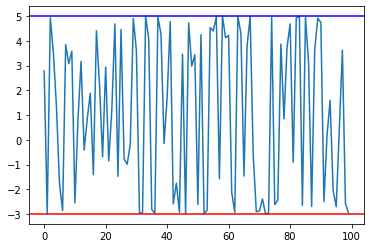
\includegraphics[width=\textwidth/2]{images/4_graph.png}
	\caption{RRQ}
	\label{fig:4:RRQ}
\end{figure}
10 vectors and their RRQs are :
\begin{align*}
	[8.79546278, 2.06447912] &\rightarrow 2.779715855809442\\
	[ 9.5063905,  -8.90054609] &\rightarrow -2.9913427706469595\\
	[7.76486343, 6.4787083 ] &\rightarrow4.935298822710415\\
	[8.980074,   3.18657326] &\rightarrow 3.521315522110756\\
	[-3.16092004, -0.13259838] &\rightarrow 1.3350048755291104\\
	[-6.54872245,  2.68558311] &\rightarrow -1.8084307457639526\\
	[-9.18640328,  7.06257587] &\rightarrow -2.8656246827096234\\
	[8.16544874, 3.41700323] &\rightarrow 3.8488780492756383\\
	[9.74184802, 2.73129675] &\rightarrow 3.079479954078956\\
	[8.5244294,  3.12348018] &\rightarrow 3.584346724232756
\end{align*}
\newpage

\section{} % Q5
\begin{align*}
	\begin{bmatrix}
		3 & -2\\
		-2 & 6
	\end{bmatrix}
		&\longrightarrow \dfrac{1}{\sqrt{5}}
		\begin{bmatrix}
			2 & -1\\
			1 & 2\\
		\end{bmatrix}
		\begin{bmatrix}
			2 & 0\\
			0 & 7
		\end{bmatrix}
		\begin{bmatrix}
			2 & -1\\
			1 & 2\\
		\end{bmatrix}^t
		\dfrac{1}{\sqrt{5}}
\end{align*}
\[ 2X^2 + 7Y^2 = 1 \]
\begin{figure}[H]
	\centering
	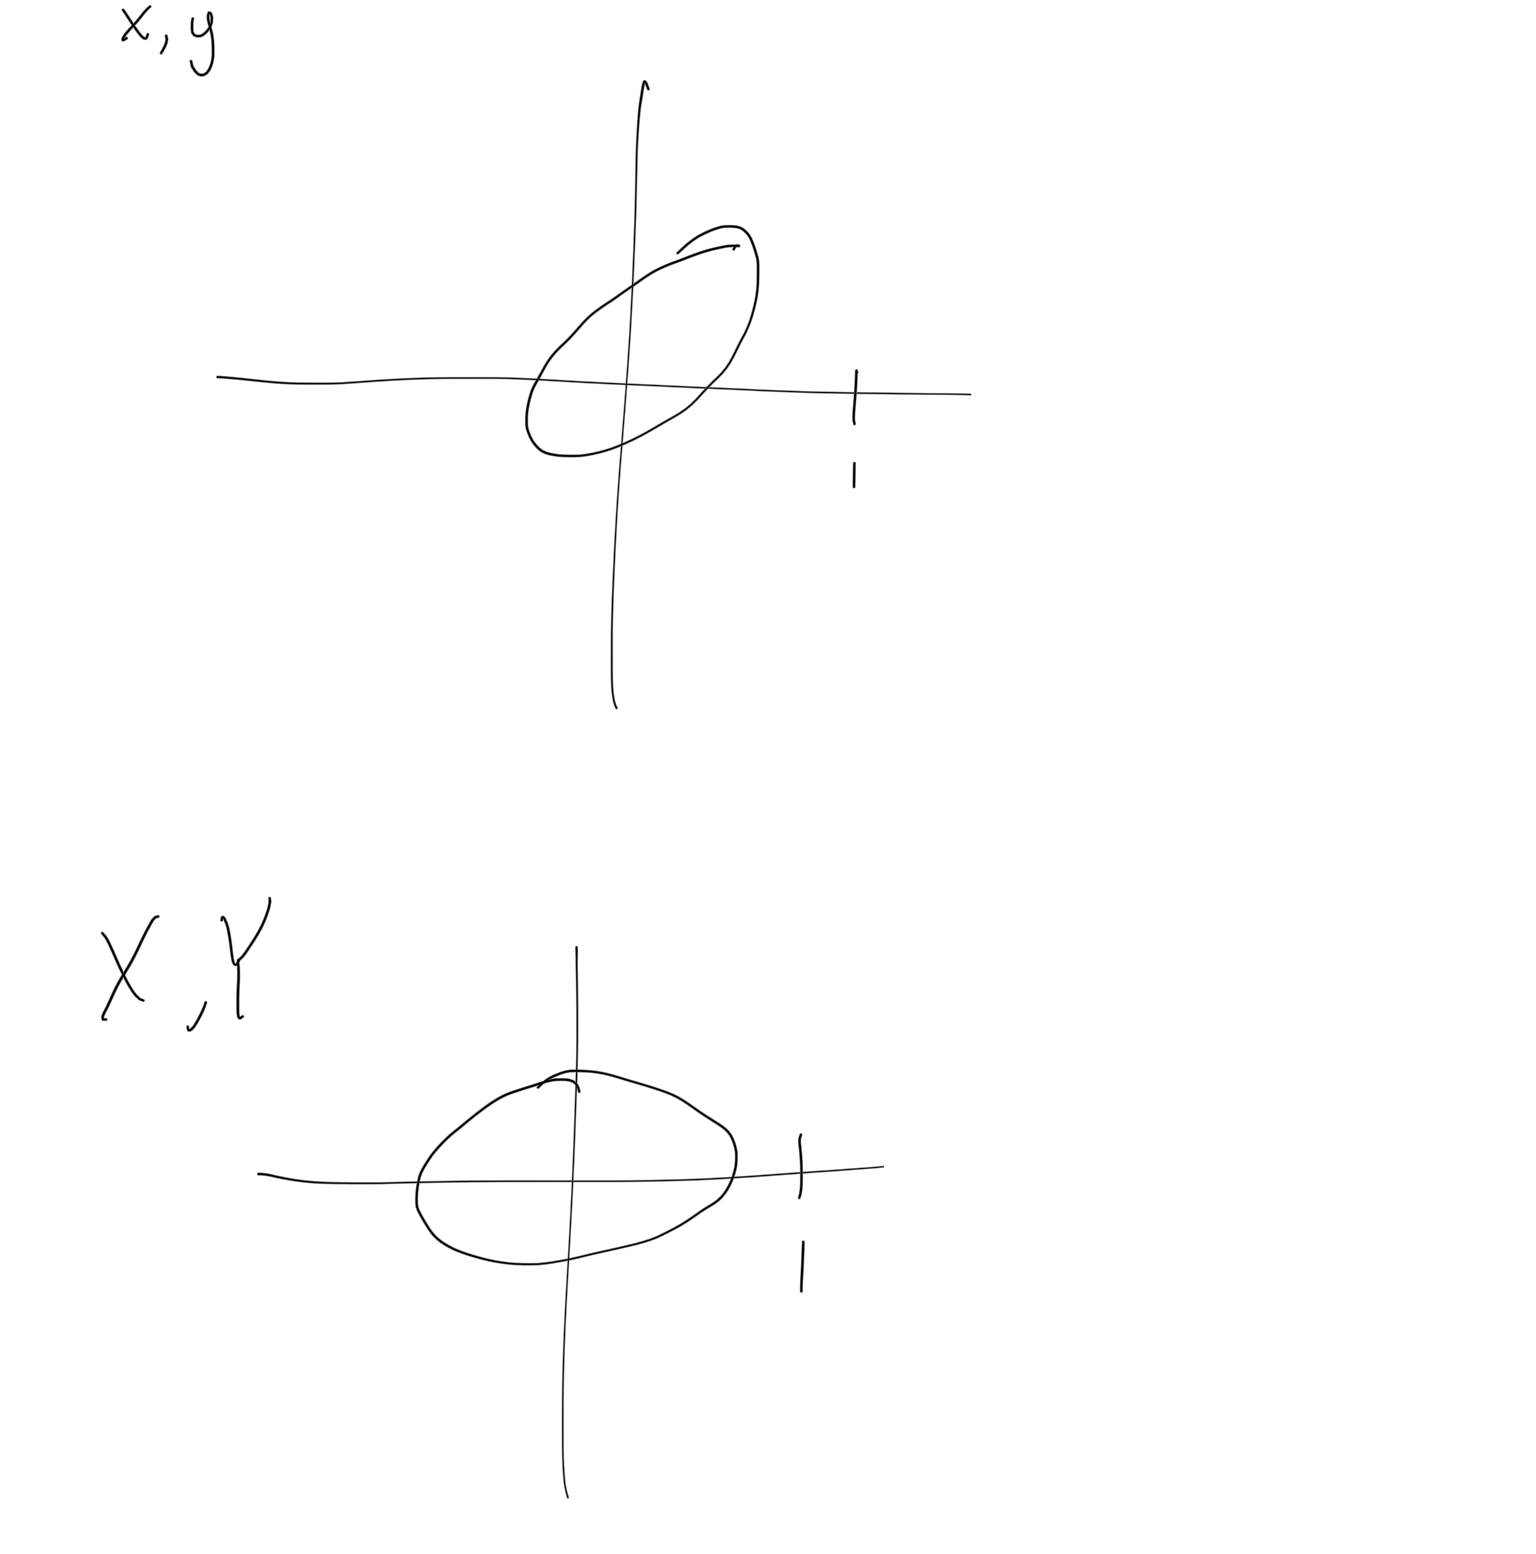
\includegraphics[width=\textwidth]{images/5.png}
	\caption{Before and After the transform}
	\label{fig:5}
\end{figure}
\newpage

\section{} % Q6
\begin{enumerate}[(a)]
	\item 
		\[
			\begin{bmatrix}
				9 & -4 & 4\\
				-4 & 7 & 0\\
				4 & 0 & 11
			\end{bmatrix}
				\longrightarrow
				\dfrac{1}{3}
				\begin{bmatrix}
					2 & -1 & -2\\
					-1 & 2 & -2\\
					2 & 2 & 1
				\end{bmatrix}
				\begin{bmatrix}
					15 & 0 & 0\\
					0 & 9 & 0\\
					0 & 0 & 3
				\end{bmatrix}
				\begin{bmatrix}
					2 & -1 & -2\\
					-1 & 2 & -2\\
					2 & 2 & 1
				\end{bmatrix}^t
				\dfrac{1}{3}
		\]
		\[ 15X^2 + 9Y^2 + 3Z^2 = 1 \]
		
	\item 
		\[ \dfrac{1}{3}
			\begin{bmatrix}
				2 & -1 & -2\\
				-1 & 2 & -2\\
				2 & 2 & 1
			\end{bmatrix}
			\begin{bmatrix}
				2 & -1 & -2\\
				-1 & 2 & -2\\
				2 & 2 & 1
			\end{bmatrix}^t
			\dfrac{1}{3} = 
			1/9
			\begin{bmatrix}
				9 & 0 & 0\\
				0 & 9 & 0\\
				0 & 0 & 9
			\end{bmatrix}
			= Id
	 	\]
\end{enumerate}
\newpage

\section{} % Q7
\begin{enumerate}[(a)]
	\item Verify that $ \sigma_{\cdots} $ is equal to its conjugate transpose.
		\begin{enumerate}
			\item [$ \sigma_x $]
				\begin{align*}
					\begin{bmatrix}
						0 & 1+0i\\
						1+0i & 0
					\end{bmatrix}
					= 
						\begin{bmatrix}
							0 & 1-0i\\
							1-0i & 0
						\end{bmatrix}
				\end{align*}
			
			\item [$ \sigma_y $]
				\begin{align*}
					\begin{bmatrix}
						0 & -i\\
						i & 0
					\end{bmatrix}
						=
						\begin{bmatrix}
							0 & -i\\
							i & 0
						\end{bmatrix}
				\end{align*}
			
			\item [$ \sigma_z $]
				\[
					\begin{bmatrix}
						1+0i & 0\\
						0 & -1+0i
					\end{bmatrix}
						=
						\begin{bmatrix}
							1-0i & 0\\
							0 & -1-0i
						\end{bmatrix}
				\]
		\end{enumerate}
	
	\item 
		\begin{enumerate}
			\item [$ \sigma_x $]
			\[
				0 + 0 = 0;\, 0*0-1*1=-1
			\]
			
			\item [$ \sigma_y $]
			\[
				0+0=0;\, 0*0--i^2=-1
			\]
			
			\item [$ \sigma_z $]
			\[
			\	1-1=0;\, 1*-1-0*0=-1
			\]
		\end{enumerate}
	
	\item \,
		\begin{enumerate}[]
			\item $ \left(\sigma_x\right)^2 = Id $
			\begin{align*}
				\begin{bmatrix}
					0 & 1\\
					1 & 0
				\end{bmatrix}
				\begin{bmatrix}
					0 & 1\\
					1 & 0
				\end{bmatrix}
				=
				\begin{bmatrix}
					1 & 0\\
					0 & 1
				\end{bmatrix}
			\end{align*}
			
			\item $ \left(\sigma_y\right)^2 = Id $
			\begin{align*}
				\begin{bmatrix}
					0 & -i\\
					i & 0
				\end{bmatrix}
				\begin{bmatrix}
					0 & -i\\
					i & 0
				\end{bmatrix}
				=
				\begin{bmatrix}
					1 & 0\\
					0 & 1
				\end{bmatrix}
			\end{align*}
			
			\item $ \left(\sigma_z\right)^2 = Id$
				\[
				\begin{bmatrix}
					1 & 0\\
					0 & -1
				\end{bmatrix}
				\begin{bmatrix}
					1 & 0\\
					0 & -1
				\end{bmatrix}
				=
				\begin{bmatrix}
					1 & 0\\
					0 & 1
				\end{bmatrix}
				\]
			\item $ \sigma_x\sigma_y = -\sigma_y\sigma_x = i\sigma_z $
				\[
					\begin{bmatrix}
						0 & 1\\
						1 & 0
					\end{bmatrix}
					\begin{bmatrix}
						0 & -i\\
						i & 0
					\end{bmatrix}
					= -
					\begin{bmatrix}
						0 & -i\\
						i & 0
					\end{bmatrix}
					\begin{bmatrix}
						0 & 1\\
						1 & 0
					\end{bmatrix}
					= i
					\begin{bmatrix}
						1 & 0\\
						0 & -1
					\end{bmatrix}
				\]
			\item $ \sigma_y\sigma_z = -\sigma_z\sigma_y = i\sigma_x $
				\[
					\begin{bmatrix}
						0 & -i\\
						i & 0
					\end{bmatrix}
					\begin{bmatrix}
						1 & 0\\
						0 & -1
					\end{bmatrix}
					=-
					\begin{bmatrix}
						1 & 0\\
						0 & -1
					\end{bmatrix}
					\begin{bmatrix}
						0 & -i\\
						i & 0
					\end{bmatrix}
					=i
					\begin{bmatrix}
						0 & 1\\
						1 & 0
					\end{bmatrix}
				\]
			\item $ \sigma_z\sigma_x = -\sigma_x\sigma_z = i\sigma_y $
				\begin{align*}
					\begin{bmatrix}
						1 & 0\\
						0 & -1
					\end{bmatrix}
					\begin{bmatrix}
						0 & 1\\
						1 & 0
					\end{bmatrix}
					=-
					\begin{bmatrix}
						0 & 1\\
						1 & 0
					\end{bmatrix}
					\begin{bmatrix}
						1 & 0\\
						0 & -1
					\end{bmatrix}
					=
					\begin{bmatrix}
						0 & -i\\
						i & 0
					\end{bmatrix}
				\end{align*}			
		\end{enumerate}
	
	\item 
		\begin{align*}
			&a
				\begin{bmatrix}
					0 & 1\\
					1 & 0
				\end{bmatrix}
				+b
				\begin{bmatrix}
					0 & -i\\
					i & 0
				\end{bmatrix}
				+c
				\begin{bmatrix}
					1 & 0\\
					0 & -1
				\end{bmatrix}\\
			&
				\begin{bmatrix}
					0 & a\\
					a & 0
				\end{bmatrix}
				+
				\begin{bmatrix}
					0 & -bi\\
					bi & 0
				\end{bmatrix}
				+
				\begin{bmatrix}
					c & 0\\
					0 & -c
				\end{bmatrix}\\
			&
				\begin{bmatrix}
					c & a-bi\\
					a+bi & -c
				\end{bmatrix}
		\end{align*}
		The trace is $ c-c = 0 $.
		\begin{align*}
			det\left(\begin{bmatrix}
				c & a-bi\\
				a+bi & c
			\end{bmatrix}\right) &= c^2 - (a-bi)(a+bi)\\
			&= -c^2 -a^2 -b^2\\
			&= -(a^2+b^2+c^2)\\
			&= -(1)\\
			&= -1
		\end{align*}
		The determinant is -1.
	
	\item [(f)] [Note: Looks like you skipped (e)]\par
		Let 
		$ A = \begin{bmatrix}
			a & b+0i\\
			b+0i & -a
		\end{bmatrix} $
		, where $ a,b $ are real. 
		The trace is $ a-a=0 $, and it's also a Hermitian matrix because it's symmetric and real. 
		The determinant is $ -a^2 -b^2 =-1$. 
		All Hermitian matrices meeting our requirements will be of this form. 
		The eigenvalues of this matrix are 
		\begin{align*}
			det\left(
				\begin{bmatrix}
					a-\lambda & b\\
					b & -a-\lambda
				\end{bmatrix}
				\right) &= (a-\lambda)(-a-\lambda)-b^2 = 0 \\
			&=  -a^2-b^2+\lambda^2 = 0\\
			\lambda^2 &= a^2+b^2\\
			\lambda^2 &= 1\\
			\lambda &= \pm 1\\
			&\qed
		\end{align*}

		
		
\end{enumerate}


\end{document}